\section{SCGRA Design} 
One key idea of the proposed design methodology is to rely on an intermediate SCGRA layer to improve compilation time of the high-level user application.  While the exact design of this SCGRA does not affect the compilation methodology, its implementation does have a significant impact on the performance of the generated gateware.  
In this section, an instance of such SCGRA design is thus presented to demonstrate the feasibility of producing high performance gateware without incurring long compilation time.  As shown in \figref{fig:pe}, the PE of this SCGRA is highly optimized for FPGA implementation, centering its design around a hard DSP block with the addition of an instruction ROM and a multi-port data memory.  In addition, a load/store path is implemented on the PEs that are responsible for data I/O beyond the FPGA.
Using this design as a template, it is envisioned that a separate hardware design team, or the high-level compiler may be able to produce similarly high-performance SCGRA that is optimized for the targeted application domain.

%The SCGRA serves as the hardware infrastructure of the proposed HLS methodology. On one hand, it should be more flexible than traditional CGRA, so that it can meet different requirements by customizing a few sub components of the SCGRA and keep the hardware overhead small. On the other hand, it should be more general than FPGA, so that it allows us to reuse the low level optimizations such as data path pipelining and improve design productivity as well. With the two design goals in mind, a 2D Torus SCGRA template is developed. It is composed of homogeneous PEs, so we can simply focus on the PE structure. The PE structure is shown in Figure \ref{fig:pe}. It basically consists of an ALU, a ROM based instruction memory and a multiple-port data memory. To connect with the system out of the FPGA, load/store data path is added to the PEs with IO interface. Details of the PE components are illustrated in the following sections.

\label{sec:scgra}
\begin{figure}[h]
\centering
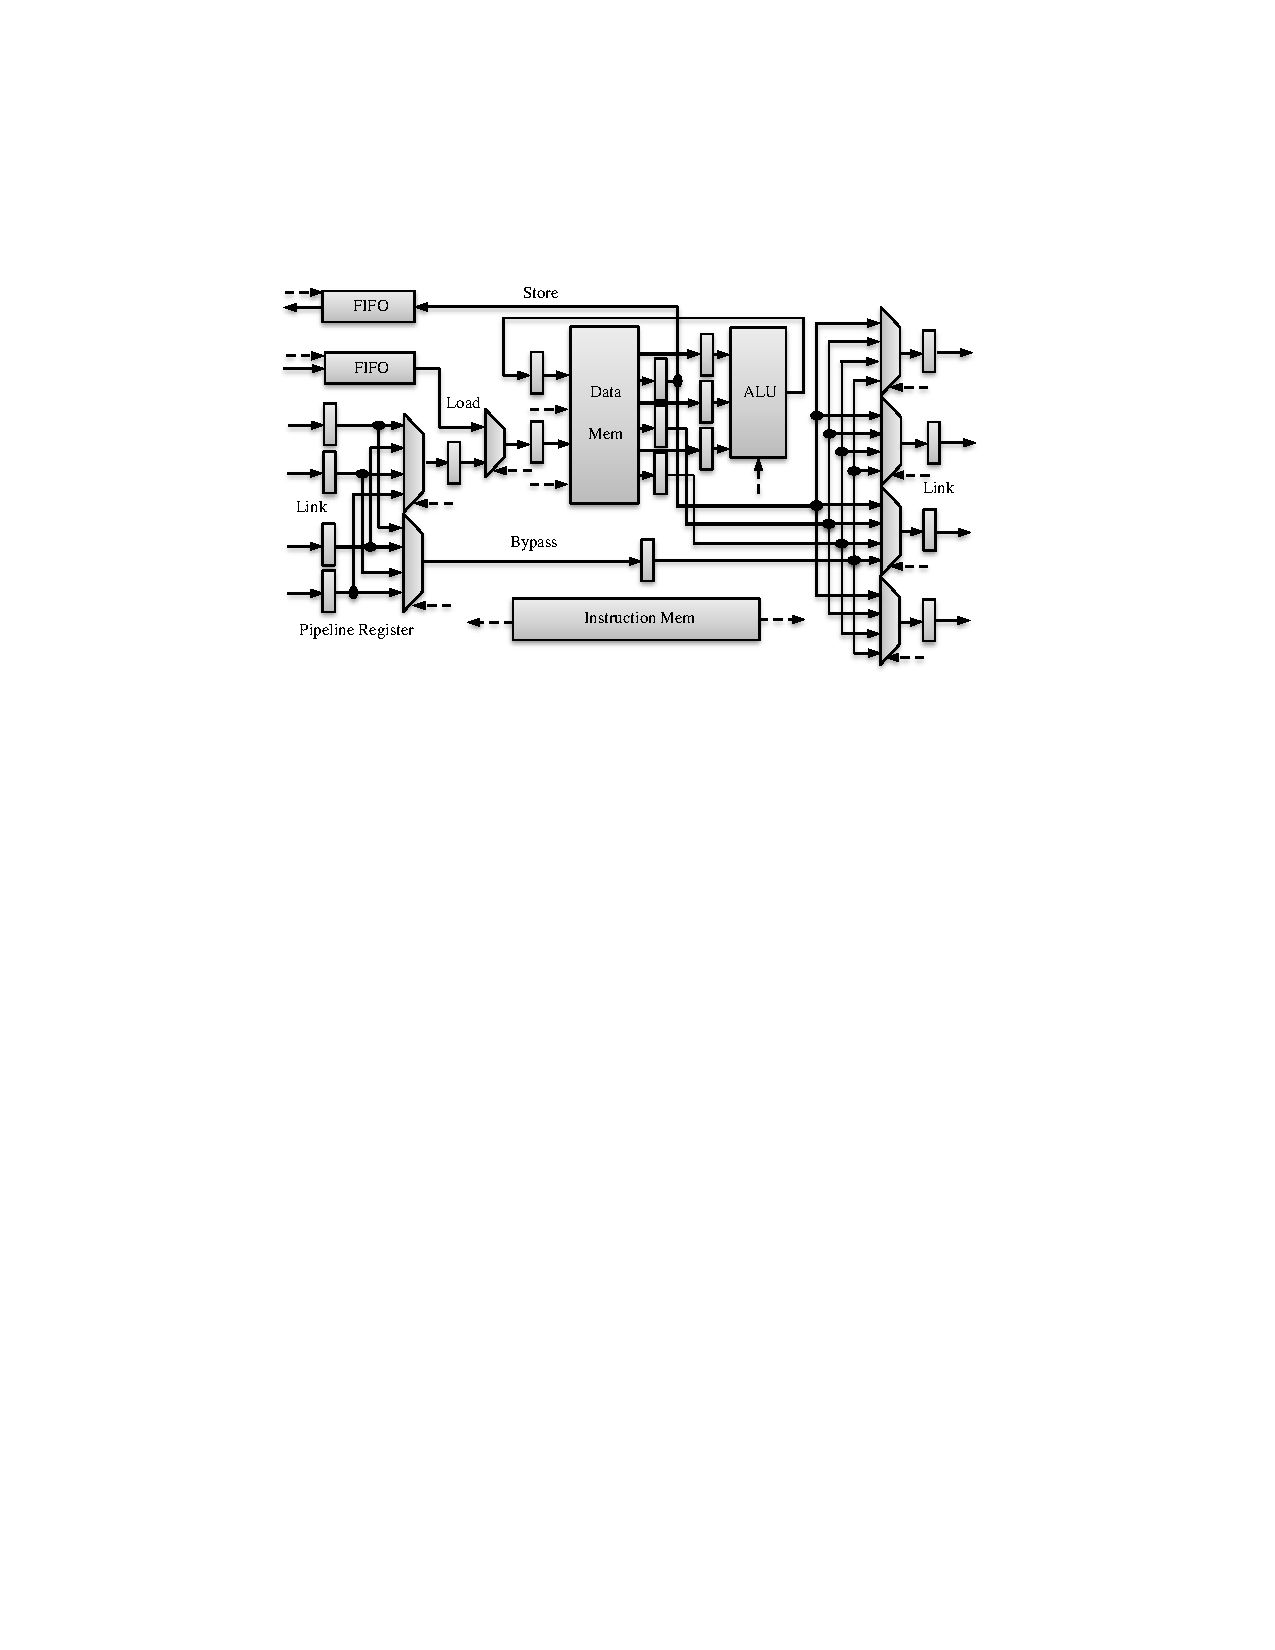
\includegraphics[width=7cm]{pe}
\vspace{-1em}
\caption{PE structure}
\label{fig:pe}
\vspace{-1em}
\end{figure}

\subsection{Instruction Memory and Data Memory}
There are two types of memory in each PE.
The instruction memory stores all the control words of the PE in each cycle.  Since its content does not change during runtime, a ROM is used to implement this instruction memory.  The content of the ROM is loaded together with the configuration bitstream.

%When the instruction memory can be implemented using a single primitive BRAM, it is able to work at extreme frequency of the FPGA device. However, the timing gets pressing when the instruction memory becomes larger. In order to improve the timing of instruction memory, the Fixed Primitives scheme is adopted when we construct the instruction memory using core generator. Meanwhile, as a single instruction is distributed to multiple primitive BRAMs, it will be better to put control bits going to the same sub components of PE such as DSP48 to the same primitive BRAM accordingly. This strategy makes the placing and routing easier and hence improves the timing. In addition, registers can be added to the output port of the instruction memory to pipeline the critical paths originated from the instruction memory.

On the other hand, data memory stores intermediate data that can either be forwarded to the PE downstream or be sent to the ALU for calculation.  For fully parallelized operation, \emph{at least} four read ports are needed -- three for the ALU and one for data forwarding.  Similarly, at least two write ports are needed to store input data from upstream memory and to store the result of the ALU in the same cycle.
Although a pair of true dual port memories may seems to be able to satisfy this port requirement, conflicts may arise if the ALU needs to read the data while the data path needs to be written.  As a result, a third dual port memory is replicated in the data memory.


%Since BRAM in Xilinx FPGA initially has read ports and write ports shared, a duplicated true dual port memory is able to satisfy the requirement. However, there will be no write port available when ALU reads data for calculation, which can't meet the needs of fully pipelined ALU. In this case, maximum ALU throughput is cut down to be 0.5. To avoid this bottleneck, we duplicate another true dual port BRAM in the data memory. Three read ports are allocated to ALU and the rest are used for forwarding.

%\begin{figure}
%\centering
%\subfloat[Two write ports and four read ports] {\label{fig:w2r4} 
%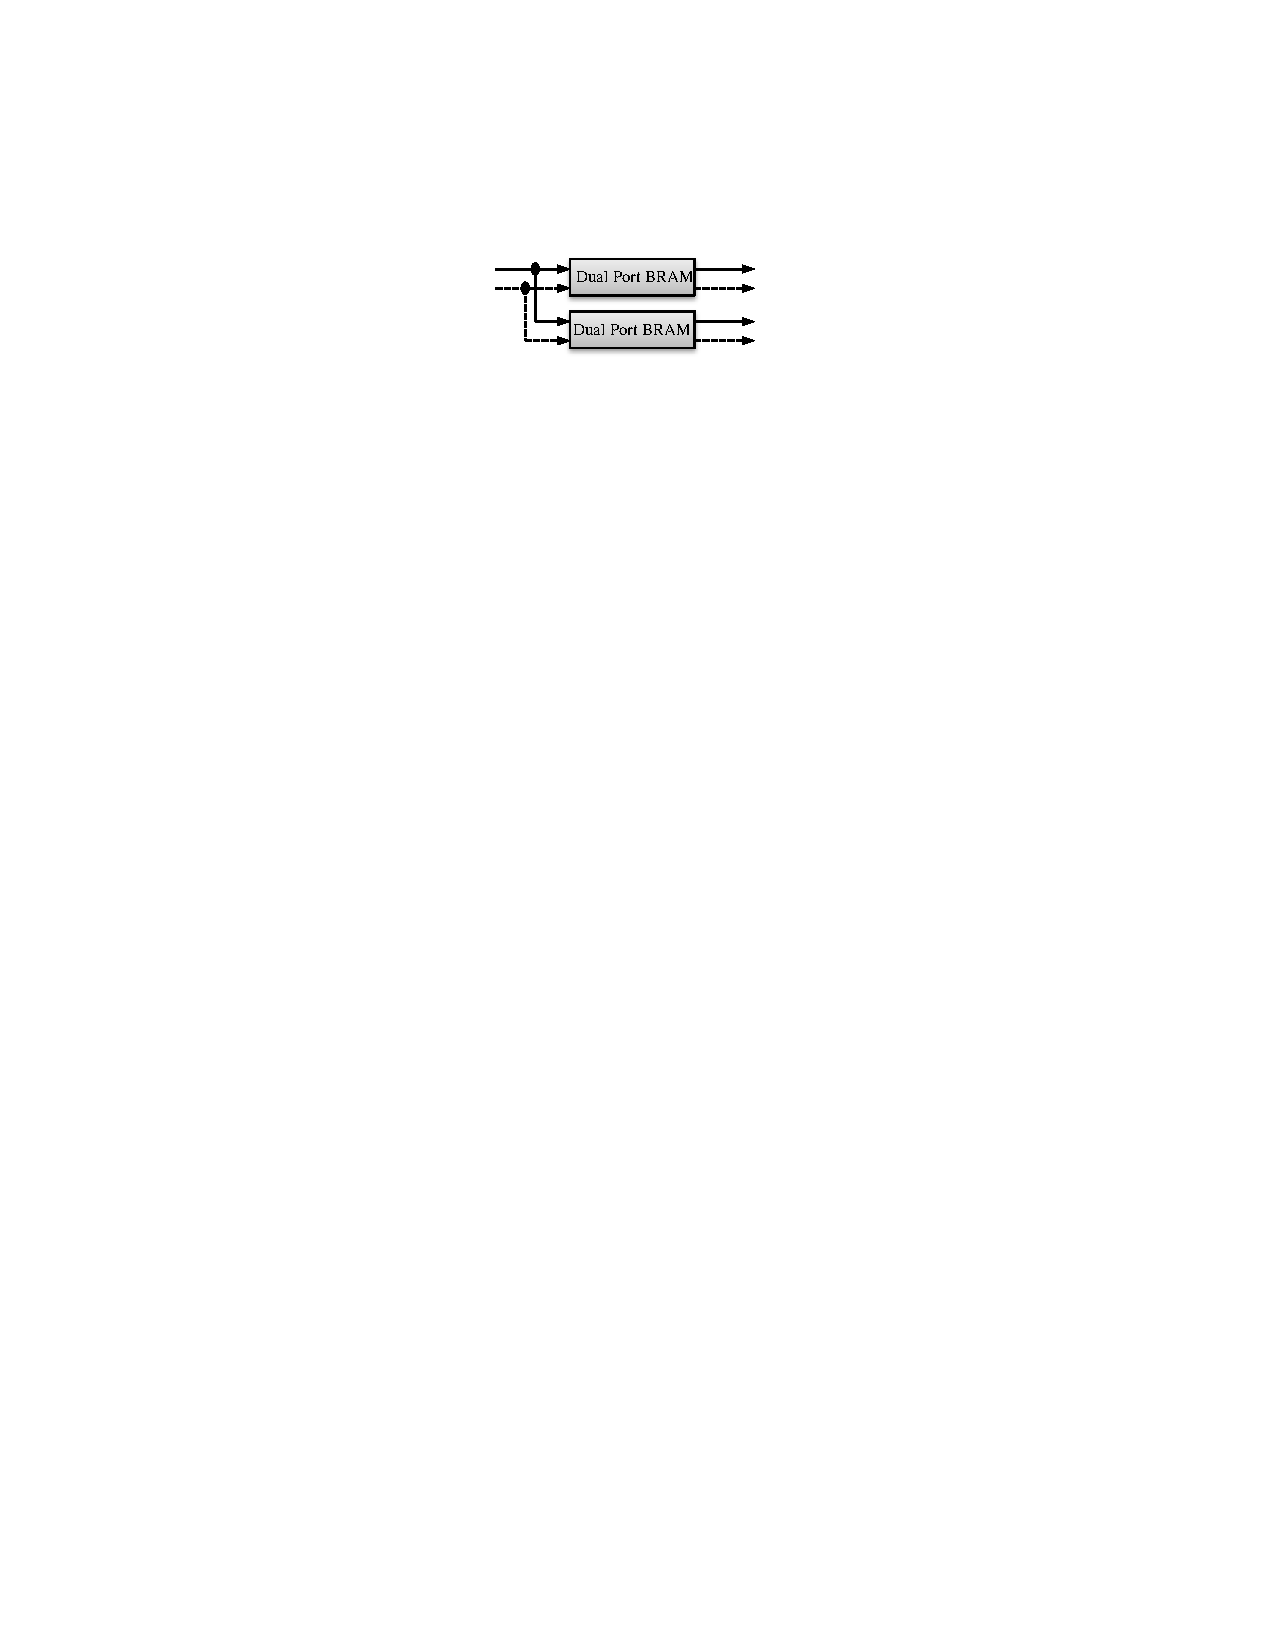
\includegraphics[width=4cm]{w2r4}}\\
%\subfloat[Three write ports and six read ports] {\label{fig:w3r6} 
%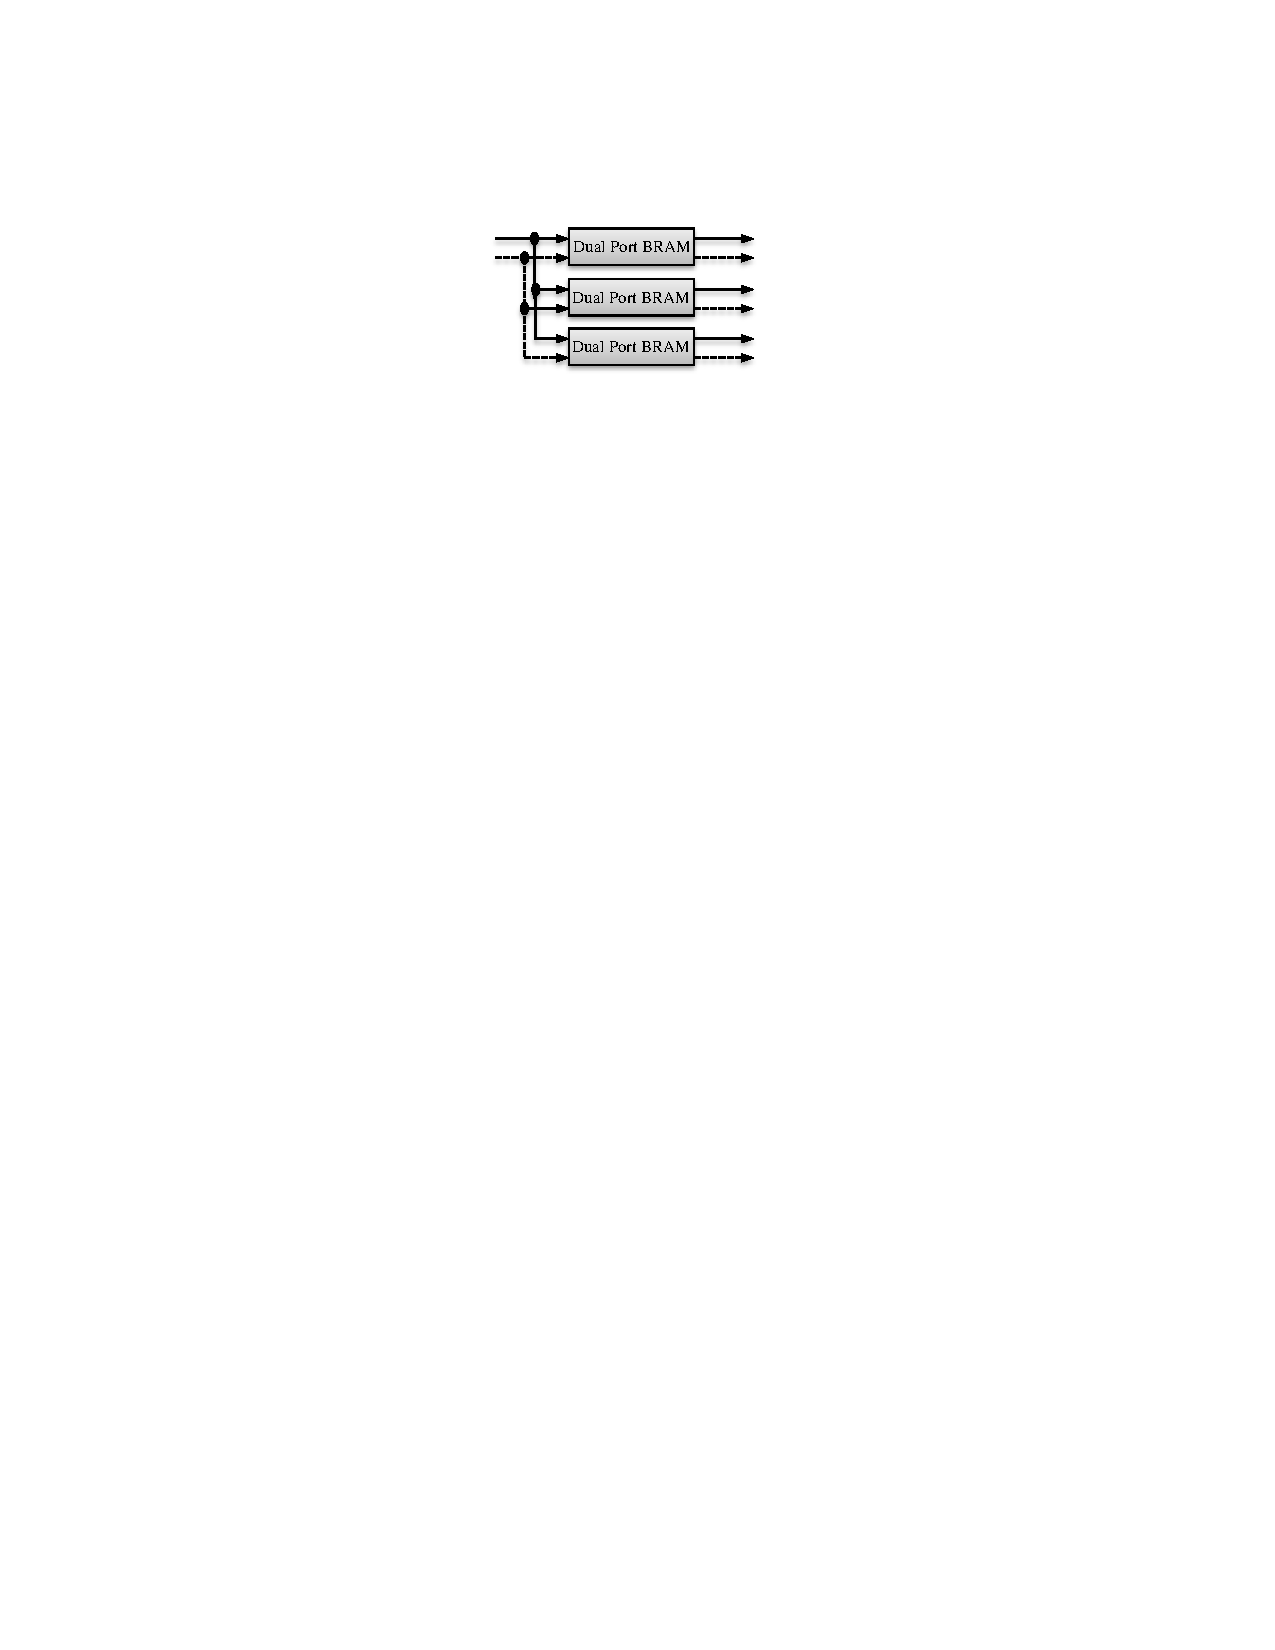
\includegraphics[width=4cm]{w3r6}}
%\caption{Multiple-port data memory}
%\label{fig:datamemory}
%\end{figure}

\subsection{ALU}
At the heart of the proposed PE is an ALU designed around the DSP core in the target Xilinx FPGA as shown in \figref{fig:ALU}.  The DSP core is responsible for all basic arithmetic operations such as multiply-add.  In addition, operations that are not provided by the DSP blocks such as add, sub and xor are handled by the 3-stage pipeline that takes the form of  $in1$ <$OP1$> $in2$ <$OP2$> $in3$.  Finally, a special PHI operation was embedded in the template to handle the applications that have branches merged. The PHI operation was implemented simply as a multiplexer, which has little influence on the final PE timing. 

%Since the proposed HLS methodology targets at computation intensive application kernels, the operations needed are basically arithmetic operations and logic operations. 
%Figure \ref{fig:ALU} shows a three-stage pipeline ALU template which is able to cover these operations. 
%DSP core in Xilinx FPGA, which has already included quite a few operations such as multiply-add, is widely used in computation applications and it is able to operate at extreme speed configured with three-stage pipeline, so we integrate it in the ALU. For the operations that are not covered, a three-stage template $in1$ <$OP1$> $in2$ <$OP2$> $in3$ is developed. $OP1$ and $OP2$ can be any operations that fit in single-stage pipeline. When $OP1$ and $OP2$ are replaced with the operations such as add, sub, and xor, the template is also able to work at full speed. In addition, we also have a special PHI operation embedded in the template to handle the applications that have branches merged. PHI operation is actually a multiplexer, so it has no influence on the timing. 

\begin{figure}
\centering
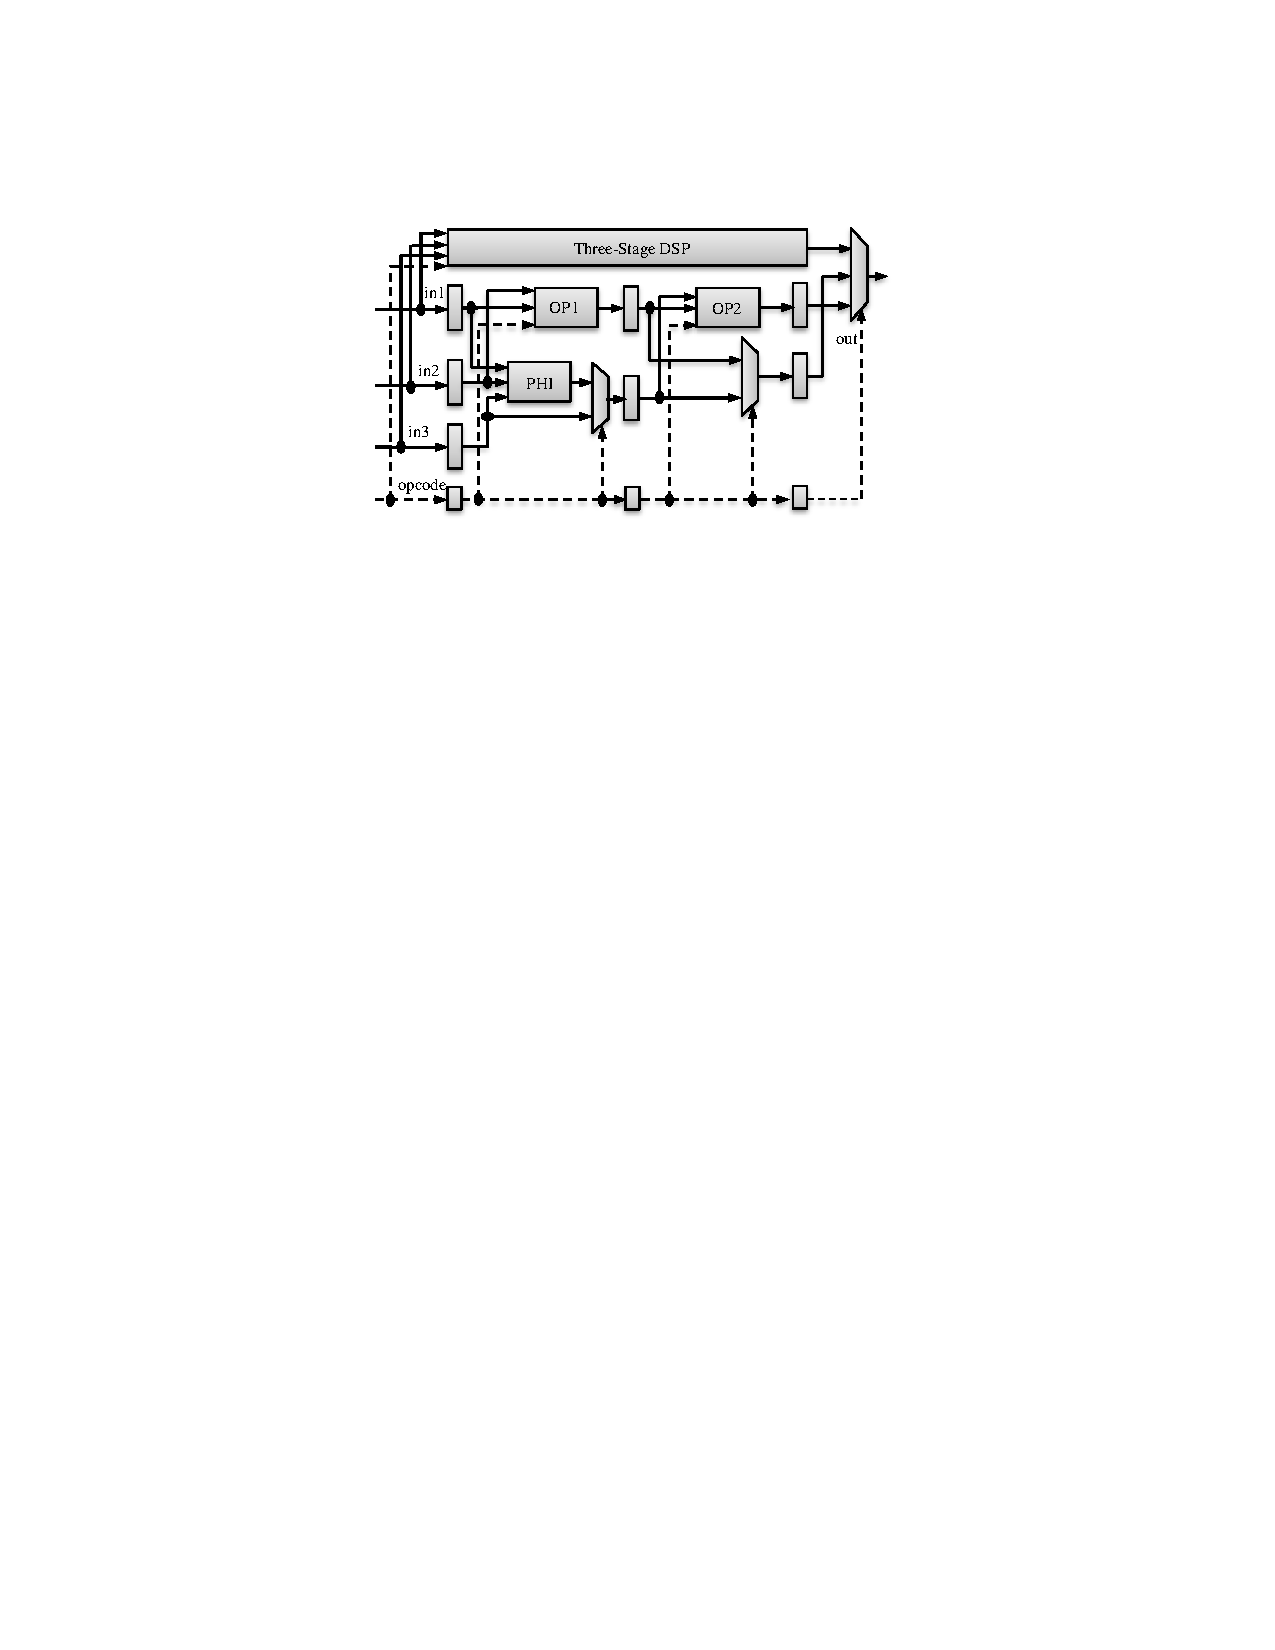
\includegraphics[width=6cm]{alu}
\vspace{-1em}
\caption{ALU Template}
\label{fig:ALU}
\vspace{-1em}
\end{figure} 

\subsection{Load/Store Interface}
For the PEs that also serve as I/O interface to the SCGRA, an additional load/store path is implemented.  In this work, the input data are assumed to be available in the scheduled order via an input FIFO.  As such, only one additional signal bit is needed to control the popping of the FIFO.   Similarly, another single bit signal is used to decide whether data should be pushed into the output FIFO.  These control bits are similarly stored using the reserved bits in the proposed instruction format.


% Since there are still reserved bits left in instruction memory, the control bits simply stored in instruction memory. Note that load path results in larger multiplexer, and additional pipeline register is added to solve this problem.
